\section{OTP}

\subsection{HMAC}

\gls{hmac} Code is an extension of a \gls{mac} and standardized in \gls{rfc}z and \gls{nist} abc.

\subsubsection{HTOP}

HMAC-based One-time Password algorithm, counter based. \gls{rfc} 899. Configurable length (6-10). Default SHA1. Truncation of HMAC

\subsubsection{TOTP}

Time based instead of counter based. \gls{rfc} 123 and \gls{oath}.


\begin{figure}[hbt]
  \centering
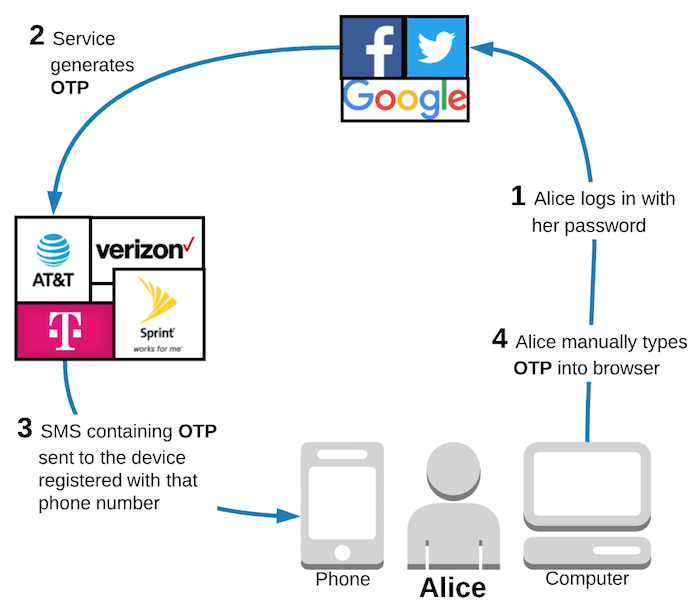
\includegraphics[width=0.8\textwidth]{pics/02---authentication-flow-3}
  \caption{}
\end{figure}

\subsubsection{pros}

\begin{enumerate}
	\item Collisions in MD5 or SHA1 are no problem, already stated/analyzed in the RFC
\end{enumerate}

\subsubsection{cons}

"Just an algorithm"

\begin{enumerate}
	\item synchronization
	\item invalidation
	\item nobody knows how the algorithm is implemented (RFC = no standard)
	\item Differences (e.g. Steam - only 5 digits, limited Alphabet)
	\item Brute Force if server does not limit
	\item Not phishing resistant
\end{enumerate}